Voici les deux plots comparatif des différentes stratégies mises en place, d'un côté (à gauche) les stratégies mises en place à notre arrivée, et de l'autre côté nos stratégies mises en place cette année.
%Afin d'évaluer l'efficacité des différentes politiques d'orchestration, les Figures 3 et 4 présentent respectivement la consommation énergétique totale et la distribution logarithmique des temps de latence. Du point de vue de la sobriété matérielle, si les heuristiques classiques (\texttt{Standard}) culminent autour de 95 000 Joules, l'approche décentralisée (\texttt{Meta\_Agent}) se détache avec une consommation exceptionnellement basse, suivie par l'algorithme hybride (\texttt{APE\_H\_Hybrid}) qui se montre le plus économe parmi les stratégies centralisées. Cependant, l'analyse du boxplot nuance cette hiérarchie en révélant que l'agent \texttt{RL\_PPO} surpasse largement toutes les autres approches en termes de réactivité applicative. En effet, bien que le \texttt{PPO} et le \texttt{DQN} consomment légèrement plus d'énergie que l'heuristique \texttt{APE\_H}, le \texttt{PPO} parvient à maintenir une écrasante majorité de ses temps d'exécution sous la barre de la seconde, évitant ainsi la forte dispersion subie par les autres stratégies. Ces résultats mettent en évidence la capacité de l'apprentissage par renforcement, et plus particulièrement du PPO, à trouver un compromis de Pareto optimal entre le respect strict des budgets de temps (SLA) et une gestion d'infrastructure énergétiquement viable.

\begin{figure}[htbp]
    \centering
    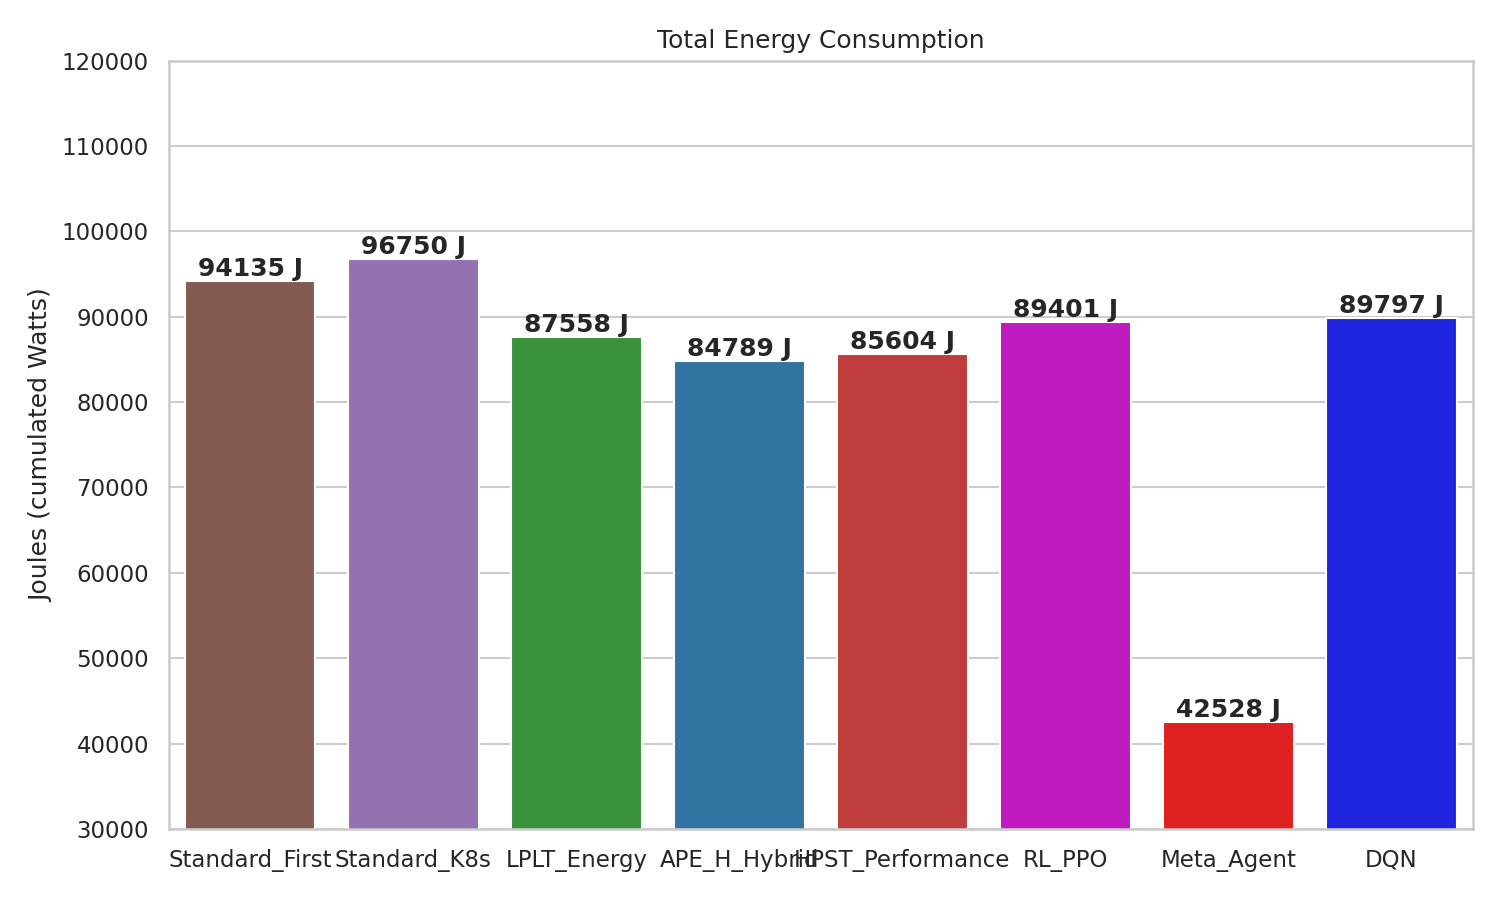
\includegraphics[width=0.8\textwidth]{images/plot_energy.png}
    \caption{Comparaison de la consommation énergétique totale des stratégies}
    \label{fig:mon_image}
\end{figure}
\begin{figure}[htbp]
    \centering
    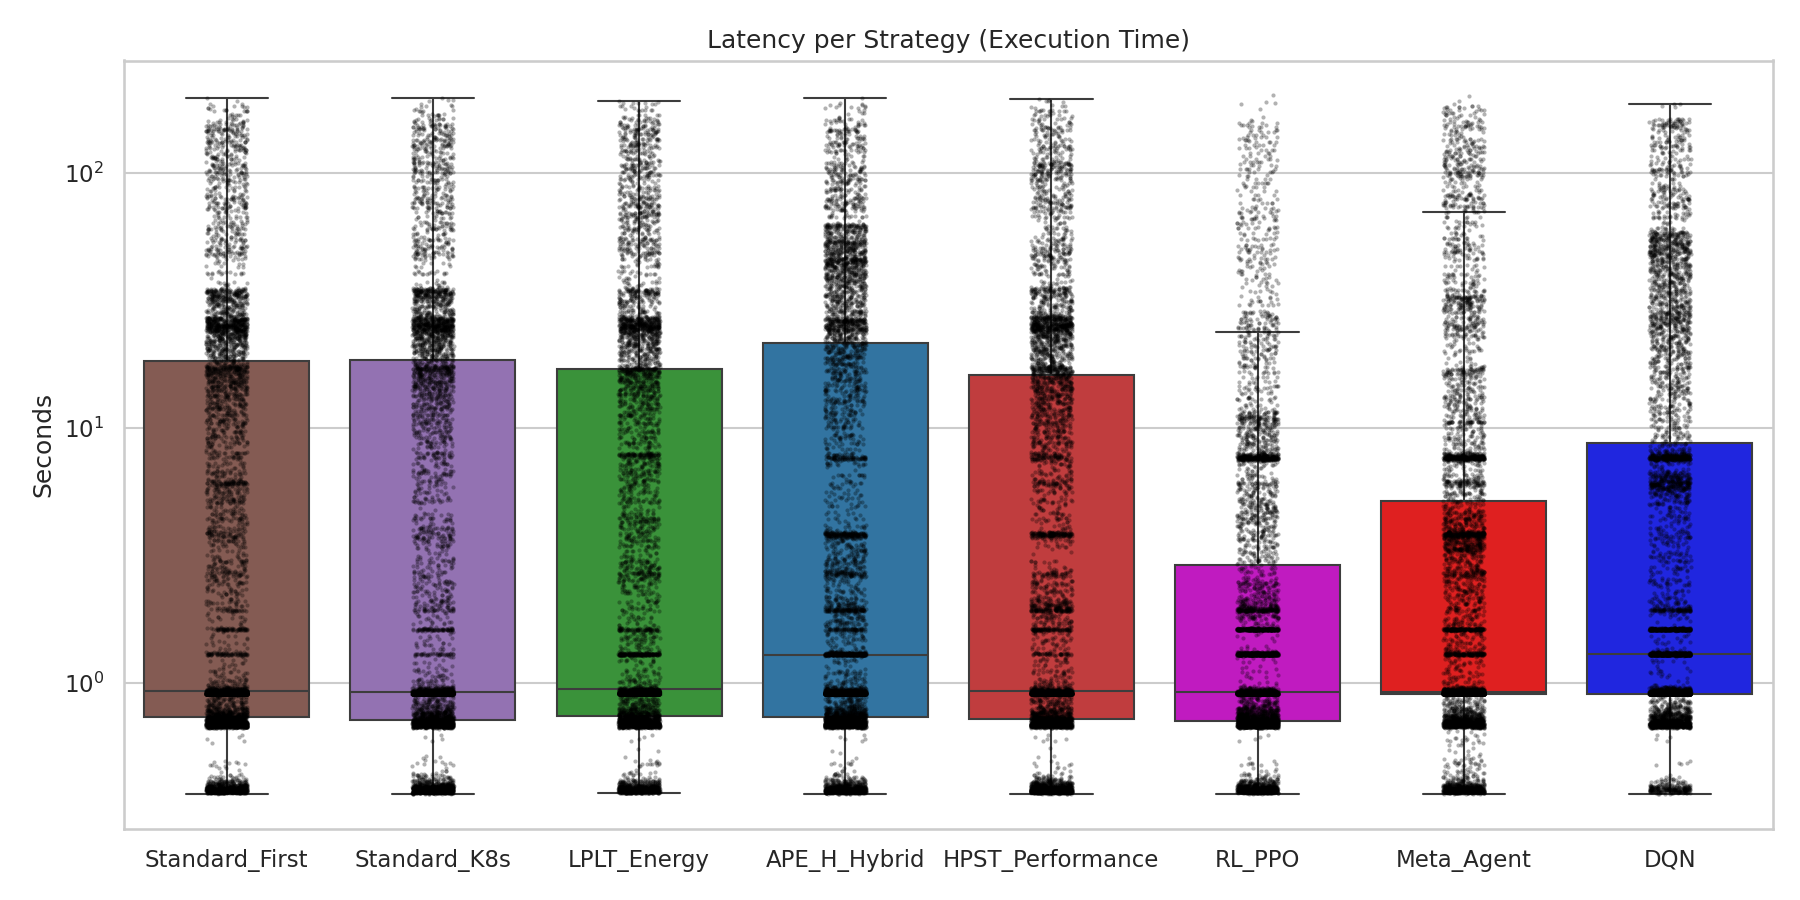
\includegraphics[width=0.8\textwidth]{images/plot_latency.png}
    \caption{Boxplot de la distribution de la latence pour chaque stratégie}
    \label{fig:mon_image}
\end{figure}

Les Figures 3 et 4 comparent l'énergie consommée et la rapidité (la latence) de nos différentes stratégies. Côté énergie, l'approche décentralisée (\texttt{Meta\_Agent}) et l'algorithme hybride (\texttt{APE\_H\_Hybrid}) sont clairement les plus économes, loin devant les méthodes classiques. Cependant, quand on regarde la rapidité sur le second graphique, l'intelligence artificielle \texttt{RL\_PPO} est de loin la plus performante. Même si elle consomme un peu plus d'énergie que les stratégies les plus écologiques, elle est la seule à traiter presque toutes les requêtes en moins d'une seconde sans jamais ralentir. En résumé, le \texttt{PPO} offre le meilleur équilibre global : il garantit des temps de réponse ultra-rapides tout en gardant une consommation électrique très raisonnable.

